\section{Results and Discussions}
	%%%%%%%%%%%%%%%%%%%%%%%%%%%%%%%%%%%%%%%%%%%%%%%%%%%%%
	In this section we are going to present some results of delamination detection and compare the conventional and the deep learning techniques.
	

	We have built two version of FCN-DensNEt models based on the output layer.
	The first model has a sigmoid function in its output layer, and the second model has a softmax function in its output layer.
	As mentioned earlier, sigmoid function produces  
	
	
	%first figure
	%%%%%%%%%%%%%%%%%%%%%%%%%%%%%%%%%%%%%%%%%%%%%%%%%%%
	\begin{figure} [h!]
		\centering
		\begin{subfigure}[b]{0.47\textwidth}
			\centering
			\includegraphics[scale=1]{RMS_flat_shell_Vz_433_500x500bottom.png}
			\caption{}
			\label{fig:dispersion0deg_direct}
		\end{subfigure}
		\hfill
		\begin{subfigure}[b]{0.47\textwidth}
			\centering
			\includegraphics[scale=1]{m1_rand_single_delam_433.png}
			\caption{}
			\label{fig:m1_rand_single_delam_433}
		\end{subfigure}
		\hfill
		\begin{subfigure}[b]{0.47\textwidth}
			\centering
			\includegraphics[scale=1]{ERMSF_flat_shell_Vz_433_500x500bottom.png}
			\caption{}
			\label{fig:ERMSF_flat_shell_Vz_433}
		\end{subfigure}
		\hfill
		\begin{subfigure}[b]{0.47\textwidth}
			\centering
			\includegraphics[scale=1]{Binary_ERMSF_flat_shell_Vz_433_500x500bottom.png}
			\caption{}
			\label{fig:dispersion45deg_direct}
		\end{subfigure}

	%	\begin{subfigure}[b]{0.47\textwidth}
	%		\centering
	%		\includegraphics[scale=1]{FCN_DenseNet_Predicted_433_sigmoid_thresholded_0.1.png}
	%		\caption{sigmoid,n(433), tr (0.1)}
	%		\label{fig:predict_433_sigmoid_tr_0.1}
	%	\end{subfigure}
		
%		\begin{subfigure}[b]{0.47\textwidth}
%			\centering
%			\includegraphics[scale=1]{FCN_DenseNet_Predicted_433_softmax.png}
%			\caption{softmax, n(433)}
%			\label{fig:predict_433_softmax}
%		\end{subfigure}
		\caption{}
		\label{fig:optimized_direct}
	\end{figure} 
	%%%%%%%%%%%%%%%%%%%%%%%%%%%%%%%%%%%%%%%%%%%%%%%%%%%
	%second figure
	%%%%%%%%%%%%%%%%%%%%%%%%%%%%%%%%%%%%%%%%%%%%%%%%%%%
	\begin{figure} [h!]
		\centering
		\begin{subfigure}[b]{0.47\textwidth}
			\centering
			\includegraphics[scale=1]{RMS_flat_shell_Vz_438_500x500bottom.png}
			\caption{}
			\label{fig:dispersion15deg_direct}
		\end{subfigure}
		\hfill
			\begin{subfigure}[b]{0.47\textwidth}
			\centering
			\includegraphics[scale=1]{m1_rand_single_delam_438.png}
			\caption{}
			\label{fig:m1_rand_single_delam_438}
		\end{subfigure}
		\hfill
		\begin{subfigure}[b]{0.47\textwidth}
			\centering
			\includegraphics[scale=1]{ERMSF_flat_shell_Vz_438_500x500bottom.png}
			\caption{}
			\label{fig:ERMSF_flat_shell_Vz_438}
		\end{subfigure}
		\hfill
		\begin{subfigure}[b]{0.47\textwidth}
			\centering
			\includegraphics[scale=1]{Binary_ERMSF_flat_shell_Vz_438_500x500bottom.png}
			\caption{}
			\label{fig:dispersion75deg_direct}
		\end{subfigure}
		\hfill
		\begin{subfigure}[b]{0.47\textwidth}
			\centering
		\includegraphics[scale=1]{FCN_DenseNet_Predicted_438_sigmoid_thresholded_0.1.png}
		\caption{sigmoid,n(438), tr (0.1)}
		\label{fig:predict_438_sigmoid_tr_0.1}
		\end{subfigure}
		\hfill
		\begin{subfigure}[b]{0.47\textwidth}
			\centering
			\includegraphics[scale=1]{FCN_DenseNet_Predicted_438_softmax.png}
			\caption{softmax, n(438)}
			\label{fig:predict_438_softmax}
		\end{subfigure}

		\caption{}
		\label{fig:predictions}
	\end{figure} 
	%%%%%%%%%%%%%%%%%%%%%%%%%%%%%%%%%%%%%%%%%%%%%%%%%%%
	% third figure
	%%%%%%%%%%%%%%%%%%%%%%%%%%%%%%%%%%%%%%%%%%%%%%%%%%%
	\begin{figure} [h!]
		\centering
		\begin{subfigure}[b]{0.47\textwidth}
			\centering
			\includegraphics[scale=1]{RMS_flat_shell_Vz_454_500x500bottom.png}
			\caption{}
			\label{fig:dispersion30deg_direct}
		\end{subfigure}
		\hfill
		\begin{subfigure}[b]{0.47\textwidth}
			\centering
			\includegraphics[scale=1]{m1_rand_single_delam_454.png}
			\caption{}
			\label{fig:m1_rand_single_delam_454}
		\end{subfigure}
		\hfill
		\begin{subfigure}[b]{0.47\textwidth}
			\centering
			\includegraphics[scale=1]{ERMSF_flat_shell_Vz_454_500x500bottom.png}
			\caption{sigmoid,n(454), tr (0.1)}
			\label{fig:ERMSF_flat_shell_Vz_454}
		\end{subfigure}
		\hfill
		\begin{subfigure}[b]{0.47\textwidth}
			\centering
			\includegraphics[scale=1]{Binary_ERMSF_flat_shell_Vz_454_500x500bottom.png}
			\caption{}
			\label{fig:dispersion90deg_direct}
		\end{subfigure}
		\hfill
		\begin{subfigure}[b]{0.47\textwidth}
			\centering
			\includegraphics[scale=1]{FCN_DenseNet_Predicted_454_sigmoid_thresholded_0.1.png}
			\caption{sigmoid,n(454), tr (0.1)}
			\label{fig:predict_454_sigmoid_tr_0.1}
		\end{subfigure}
		\hfill	
		\begin{subfigure}[b]{0.47\textwidth}
			\centering
			\includegraphics[scale=1]{FCN_DenseNet_Predicted_454_softmax.png}
			\caption{softmax, n(454)}
			\label{fig:predict_454_softmax}
		\end{subfigure}
	
	
		\caption{}
		\label{fig:predictions}
	\end{figure} 
	%%%%%%%%%%%%%%%%%%%%%%%%%%%%%%%%%%%%%%%%%%%%%%%%%%%
	

	\begin{figure} [h!]
		\centering
		\begin{subfigure}[b]{0.47\textwidth}
			\centering
			\includegraphics[scale=1]{ERMS_CFRP_teflon_3o_375_375p_50kHz_5HC_x12_15Vpp.png}
			\caption{ERMS CFRP teflon}
			\label{fig:Delamination}
		\end{subfigure}			
		\hfill
		\begin{subfigure}[b]{0.47\textwidth}
		\centering 	
		\includegraphics[scale=1]{label_CFRP_teflon_3o_375_375p_50kHz_5HC_x12_15Vpp.png}
		\caption{Ground truth} 
		\label{fig:damage_label}
		\end{subfigure}
		\hfill
		\begin{subfigure}[b]{0.47\textwidth}
			\centering
			\includegraphics[scale=1]{Predicted_Predicted_ERMS_CFRP_teflon_3o_375_375p_50kHz_5HC_x12_15Vpp_7__threshold_0.1_sigmoid.png}
			\caption{sigmoid for the output layer} 
			\label{fig:EXP_predict_sigmoid}
		\end{subfigure}
		\hfill
		\begin{subfigure}[b]{0.47\textwidth}
			\centering
			\includegraphics[scale=1]{Predicted_Predicted_ERMS_CFRP_teflon_3o_375_375p_50kHz_5HC_x12_15Vpp_7_softmax.png}
			\caption{softmax for the output layer} 
			\label{fig:EXP_predict_softmax}
		\end{subfigure}
			\caption{Experimental results}
			\label{}
		\end{figure}
	
